\section{Differential calculus}

\subsection{What is a derivative?}

Differential calculus is the study of infinitesimal variations. Consider for instance a function \(y = f(x)\). Given some interval from \(a\) and \(a+h\), we can study the variation of \(f\) in this interval by considering the ratio
%
\[
\frac{f(a+h) - f(a)}{h}\text{.}
\]
%
This is visualised in figure \ref{fig:Ch06-variation-of-f}.



\begin{figure}[H]
    \centering

    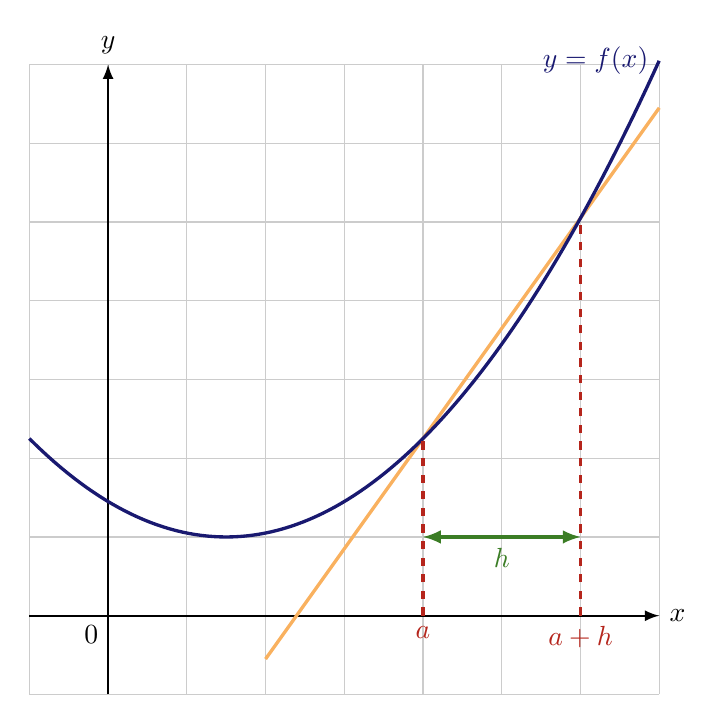
\begin{tikzpicture}[scale=1]
        \draw[thin,gray!40] (-1,-1) grid (7, 7);
        \draw[thick, ->, >=latex] (-1,0)--(7,0) node[right]{\(x\)};
        \draw[thick, ->, >=latex] (0,-1)--(0,7) node[above]{\(y\)};
        \draw (0, 0) node[below left] {0};

        \draw[BurntOrange!60, very thick, domain=2:7] plot (\x,{1.4*\x - 3.35});

        \draw [MidnightBlue, very thick, domain=-1:7, samples=100] plot (\x,{0.2*(\x-1.5)^2 + 1}) node[left, MidnightBlue] {\(y = f(x)\)};

        \draw[BrickRed, very thick, dashed] (4, 0) node[below] {\(a\)} -- (4, {0.2*(4-1.5)^2 + 1});

        \draw[BrickRed, very thick, dashed] (6, 0) node[below] {\(a+h\)} -- (6, {0.2*(6-1.5)^2 + 1});

        \draw[OliveGreen, very thick, latex-latex] (4, 1) -- (6, 1) node[pos=0.5, below] {\(h\)};
    \end{tikzpicture}
    
    \caption{Studying the variation of a function \(f\) between \(x = a\) and \(x = a + h\). The ratio \(\frac{f(a+h)-f(a)}{h}\) can be visualised as the slope of the orange line which passes through the points \((a, f(a))\) and \((a+h, f(a+h))\).}
    \label{fig:Ch06-variation-of-f}
\end{figure}



To study the variations close to \(a\), we consider the limit of this ratio as \(h\) tends to zero. See figure \ref{fig:Ch06-derivative-of-f}.
%
\[
\lim_{h\to 0} \frac{f(a+h) - f(a)}{h}
\]
%
This limit is referred to as the \textit{derivative} of \(f\) in \(a\). If this limit exists, then the function \(f\) is said to be \textit{differentiable} in \(a\).



\begin{figure}[H]
    \centering

    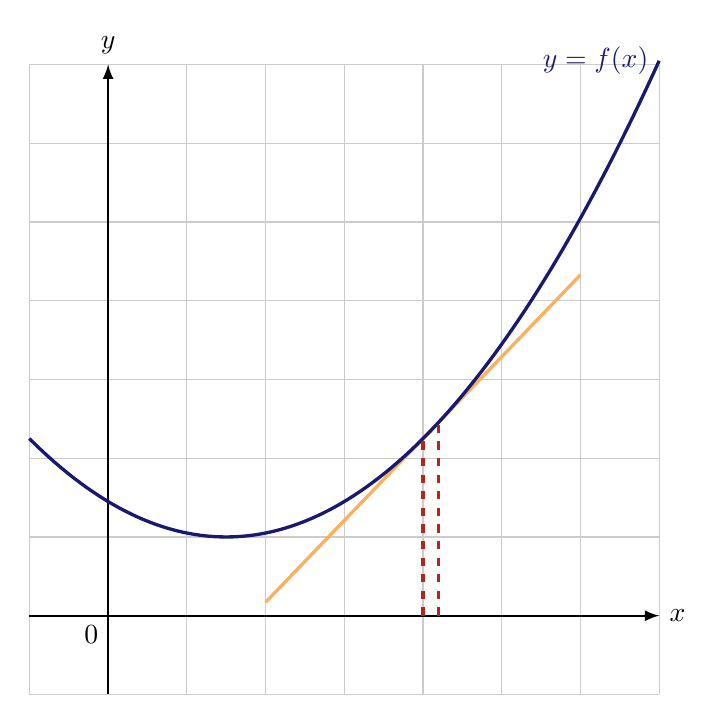
\begin{tikzpicture}[scale=1]
        \draw[thin,gray!40] (-1,-1) grid (7, 7);
        \draw[thick, ->, >=latex] (-1,0)--(7,0) node[right]{\(x\)};
        \draw[thick, ->, >=latex] (0,-1)--(0,7) node[above]{\(y\)};
        \draw (0, 0) node[below left] {0};

        \draw[BurntOrange!60, very thick, domain=2:6] plot (\x,{1.04*\x-1.91});

        \draw [MidnightBlue, very thick, domain=-1:7, samples=100] plot (\x,{0.2*(\x-1.5)^2 + 1}) node[left, MidnightBlue] {\(y = f(x)\)};

        \draw[BrickRed, very thick, dashed] (4, 0) -- (4, {0.2*(4-1.5)^2 + 1});

        \draw[BrickRed, very thick, dashed] (4.2, 0) -- (4.2, {0.2*(4.2-1.5)^2 + 1});
    \end{tikzpicture}
    
    \caption{To find the derivative of a function \(f\) in \(a\), we consider the slope of the orange line as the length of the interval \(h\) tends to zero.}
    \label{fig:Ch06-derivative-of-f-as-limit}
\end{figure}



\begin{figure}[H]
    \centering

    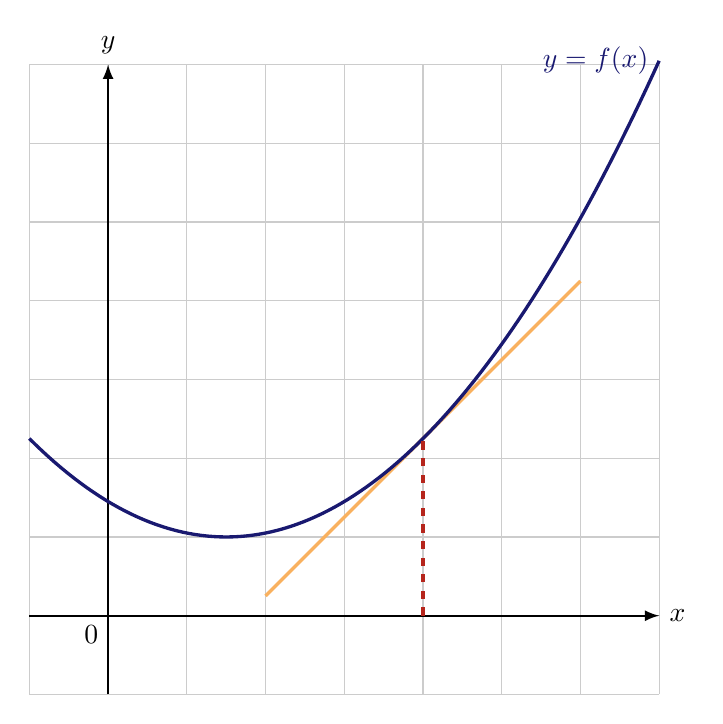
\begin{tikzpicture}[scale=1]
        \draw[thin,gray!40] (-1,-1) grid (7, 7);
        \draw[thick, ->, >=latex] (-1,0)--(7,0) node[right]{\(x\)};
        \draw[thick, ->, >=latex] (0,-1)--(0,7) node[above]{\(y\)};
        \draw (0, 0) node[below left] {0};

        \draw[BurntOrange!60, very thick, domain=2:6] plot (\x,{\x-1.75});

        \draw [MidnightBlue, very thick, domain=-1:7, samples=100] plot (\x,{0.2*(\x-1.5)^2 + 1}) node[left, MidnightBlue] {\(y = f(x)\)};

        \draw[BrickRed, very thick, dashed] (4, 0) -- (4, {0.2*(4-1.5)^2 + 1});
    \end{tikzpicture}
    
    \caption{The derivative of a function \(f\) in a point \(a\) can be thought of as the slope of the tangent to the graph of \(f\) at the point where \(x = a\).}
    \label{fig:Ch06-derivative-of-f-as-tangent}
\end{figure}


The derivative of a function \(f\) in some value \(a\) is denoted as \(f'(a)\).

Note that the derivative of \(f\) is itself a function, which is denoted here as \(f'\). We can also write this as
%
\[\frac{df}{dx} \text{\;\;or\;\;} f^{(1)}\text{.}\]
%
Note that \(\frac{df}{dx}\) is not a quotient or fraction. It can be read as applying a differentiation operator \(\frac{d}{dx}\) to a function \(f\). The differentiation operator specifies the variable of differentiation, which in this case is \(x\).

Note that
%
\begin{itemize}
    \item If the derivative of a function \(f\) is \(g\), i.e.
    %
    \[f' = g\]
    %
    then \(f\) is called the \textit{primitive} or \textit{antiderivative} of \(g\).

    \item Applying the differentiation operator to a function \(f\) twice, i.e.
    %
    \[\frac{d}{dx} \left(\frac{df}{dx}\right)\]
    %
    can be written more compactly as
    %
    \[\frac{d^2 f}{dx^2}\text{.}\]
    %
    This produces a \textit{second-order derivative}, which is denoted as \(f''(x)\) or \(f^{(2)}(x)\).
\end{itemize}



\subsection{Finding the derivative of a function}

To find the derivative of a function, we can use the definition of the derivative as a limit. Consider for instance the function \(f(x) = x^2\). We can find the derivative of \(f\) by computing the limit
%
\begin{align*}
    \lim_{h \to 0} \frac{f(x+h) - f(x)}{h} &= \lim_{h \to 0} \frac{(x + h)^2 - x^2}{h}\\
    &= \lim_{h \to 0} \frac{x^2 + 2hx + h^2 - x^2}{h}\\
    &= \lim_{h \to 0} \frac{2hx + h^2}{h}\\
    &= \lim_{h \to 0} (2x + h)\\
    &= \lim_{h \to 0} 2x\\
    &= 2x
\end{align*}
%
which means that the derivative of \(f(x) = x^2\) at any point \(a\) is given by \(f'(a) = 2a\). In other words, the tangent to the graph of \(f(x)\) when \(x = a\) must have a slope of \(2a\).



\begin{figure}[H]
    \centering

    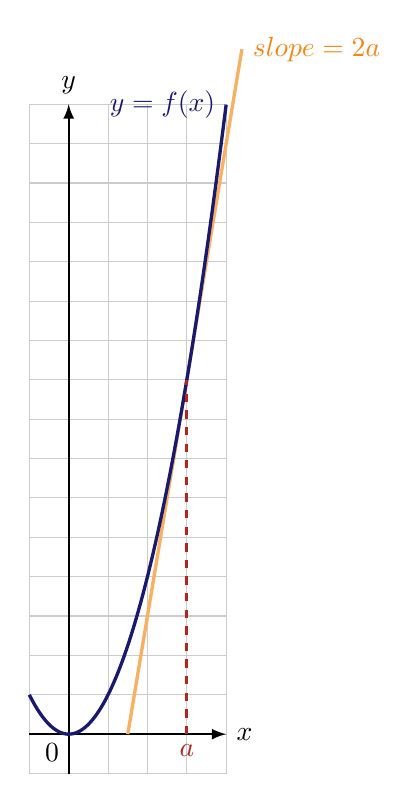
\begin{tikzpicture}[scale=0.5]
        \draw[thin,gray!40] (-1,-1) grid (4, 16);
        \draw[thick, ->, >=latex] (-1,0)--(4,0) node[right]{\(x\)};
        \draw[thick, ->, >=latex] (0,-1)--(0,16) node[above]{\(y\)};
        \draw (0, 0) node[below left] {0};

        \draw[BurntOrange!60, very thick, domain=1.5:4.4] plot (\x,{6*\x-9}) node[right, BurntOrange] {\(\text{slope} = 2a\)};

        \draw [MidnightBlue, very thick, domain=-1:4, samples=100] plot (\x,{(\x)^2}) node[left, MidnightBlue] {\(y = f(x)\)};

        \draw[BrickRed, very thick, dashed] (3, 0) node[below, BrickRed] {\(a\)} -- (3, 9);
    \end{tikzpicture}
    
    \caption{The derivative of \(x^2\) is \(2x\). This means the derivative of \(x^2\) (or the slope of the tangent to the graph of \(y = x^2\)) at any point \(a\) is \(2a\).}
    \label{fig:Ch06-derivative-of-f-as-tangent}
\end{figure}

Finding derivatives as a limit can be cumbersome and tedious. To speed this up, it might be helpful to memorise a few differentiation rules, as listed below. Here, \(f\) and \(g\) are differentiable functions, \(c\) is a constant, and \(n\) is any real number.
%
\newcommand{\reddiffarrow}{{\;\;\color{BrickRed}\xrightarrow{\frac{d}{dx}}\;\;}}
%
\begin{align}
    c &\reddiffarrow 0\\
    x &\reddiffarrow 1\\
    \sin{x} &\reddiffarrow \cos{x}\\
    \cos{x} &\reddiffarrow -\sin{x}\\
    e^x &\reddiffarrow e^x\\
    \ln{x} &\reddiffarrow \frac{1}{x}\\
    f(x) \pm g(x) &\reddiffarrow f'(x) \pm g'(x) \label{eq:Ch06-diff-additivity}\\
    c\cdot f(x) &\reddiffarrow c\cdot f'(x) \label{eq:Ch06-diff-mult-by-constant}\\
    x^n &\reddiffarrow n x^{n-1} \label{eq:Ch06-power-rule}\\
    f(x) \cdot g(x) &\reddiffarrow f(x) \cdot g'(x) + g(x) \cdot f'(x) \label{eq:Ch06-product-rule}\\
    \frac{f(x)}{g(x)} &\reddiffarrow \frac{g(x) \cdot f'(x) - f(x) \cdot g'(x)}{(g(x))^2} \label{eq:Ch06-quotient-rule}\\
    f(g(x)) &\reddiffarrow f'(g(x)) \cdot g'(x) \label{eq:Ch06-chain-rule}
\end{align}

Several notes:
%
\begin{itemize}
    \item From equation \eqref{eq:Ch06-diff-additivity} we have
    %
    \[f(x) + g(x) \reddiffarrow f'(x) + g'(x)\text{.}\]
    %
    Combining this with equation \eqref{eq:Ch06-diff-mult-by-constant} we see that differentiation is a linear operation.

    \item The power rule (equation \eqref{eq:Ch06-power-rule}) can be applied with any real number \(n\). A few examples are shown below.
    %
    \begin{align*}
        \frac{1}{x} = x^{-1} &\reddiffarrow -x^{-2} = -\frac{1}{x^2}\\
        \sqrt{x} = x^{\frac{1}{2}} &\reddiffarrow \frac{1}{2} x^{-\frac{1}{2}} = \frac{1}{2\sqrt{x}}
    \end{align*}

    \item The quotient rule (equation \eqref{eq:Ch06-quotient-rule}) can be derived from the power rule (equation \eqref{eq:Ch06-power-rule}), the product rule (equation \eqref{eq:Ch06-product-rule}), and the chain rule (equation \eqref{eq:Ch06-chain-rule}).
\end{itemize}


An example problem is shown below.


\vspace{15pt}
\begin{mdframed}[linewidth=1pt]

\noindent \textbf{Problem.} Calculate \(\dfrac{d}{dx}\; 3e^{x^2 + 2}\).

\textbf{Solution 1.} Let \(f(x) = 3e^x\) and \(g(x) = x^2 + 2\). We want to find \(\frac{d}{dx} f(g(x))\).

Note that \(f'(x) = 3e^x\) and \(g'(x) = 2x\). Hence, we have
%
\begin{align*}
    \frac{d}{dx} f(g(x)) &= f'(g(x)) \cdot g'(x) \tag{chain rule}\\
    &= f'(x^2 + 2) \cdot 2x\\
    &= 3e^{x^2 + 2} \cdot 2x\\
    &= 6xe^{x^2 + 2}\text{.}
\end{align*}


\textbf{Solution 2.} Those who are more fluent with the rules of differentiation can simply apply the rules to find:
%
\begin{align*}
    \frac{d}{dx} 3e^{x^2 + 2} &= 3 \cdot \left(e^{x^2 + 2}\right) \cdot (2x)\\
    &= 6xe^{x^2 + 2}\text{.}
\end{align*}

\vspace{2pt}
\end{mdframed}

Generalising from this example problem, we can show that a function of the form
%
\begin{equation*}
    f(x) = c \cdot e^{g(x)} \tag{where \(c\) is a constant}
\end{equation*}
%
must have the derivative
%
\begin{align*}
    f'(x) &= c \cdot e^{g(x)} \cdot g'(x)\\
    &= f(x) \cdot g'(x)\text{.}
\end{align*}
%
This will be useful for solving differential equations later.




\subsection{More on differentiability}

Recall that a function \(f(x)\) is said to be differentiable if the derivative of \(f'(x)\) exists when \(x = a\).

We note the following theorem.
%
\begin{quote}
    \textbf{Differentiability is stronger than continuity.}

    If a function \(f\) is differentiable in \(a\), then \(f\) is continuous in \(a\).
\end{quote}
%
We can prove this as follows.
%
\begin{quote}
    \textbf{Proof that differentiability implies continuity.}

    We assume differentiability, meaning that the limit
    %
    \[f'(a) = \lim_{h \to 0} \frac{f(a + h) - f(a)}{h}\]
    %
    exists. We want to prove that
    %
    \[\lim_{x \to a} f(x) = f(a)\text{.}\]

    Consider the following limit.
    %
    \begin{align*}
        \lim_{x \to a} (f(x) - f(a)) &= \lim_{x \to a} \left((f(x) - f(a)) \cdot \frac{x - a}{x - a} \right) \tag{\(\because x - a \neq 0\)}\\
        &= \lim_{x \to a} \left(\frac{f(x) - f(a)}{x - a} \cdot (x - a) \right)\\
        &= \left(\lim_{x \to a} \frac{f(x) - f(a)}{x - a}\right) \cdot \left(\lim_{x \to a} (x - a)\right) \\
        &= f'(a) \cdot 0\\
        &= 0
    \end{align*}
    %
    Rearranging, we get
    %
    \[\lim_{x \to a} f(x) = f(a)\]
    %
    which concludes the proof.
\end{quote}

Intuitively, we can think of differentiability as whether the tangent to the graph of a function \(f\) at a point \(a\) exists. For instance, the absolute value function \(\abs{x}\) is not differentiable at \(x = 0\) because at \(x = 0\), the graph of \(y = \abs{x}\) consists of a sharp angular point where no tangent can be drawn. See figure \ref{fig:Ch06-abs-non-differentiable}.

\begin{figure}[H]
    \centering

    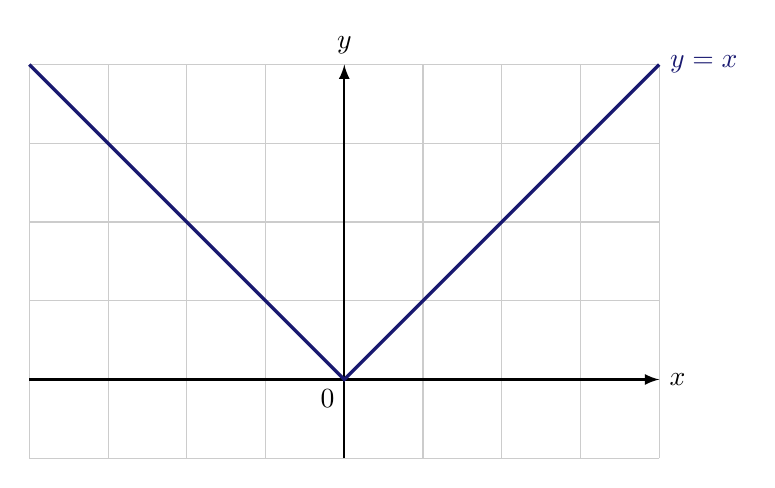
\begin{tikzpicture}[scale=1]
        \draw[thin,gray!40] (-4,-1) grid (4, 4);
        \draw[thick, ->, >=latex] (-4,0)--(4,0) node[right]{\(x\)};
        \draw[thick, ->, >=latex] (0,-1)--(0,4) node[above]{\(y\)};
        \draw (0, 0) node[below left] {0};

        \draw[MidnightBlue, very thick, domain=-4:4] plot (\x,{abs(\x)}) node[right] {\(y = \abs{x}\)};
    \end{tikzpicture}
    
    \caption{The absolute value function is non-differentiable at \(x = 0\).}
    \label{fig:Ch06-abs-non-differentiable}
\end{figure}




\subsection{Stationary points}

If we have \(\frac{df}{dx} > 0\) at some point \(a\), we say that \(f\) is \textit{increasing} at that point. Conversely, if we have \(\frac{df}{dx} < 0\) at some point \(a\), we say that \(f\) is \textit{decreasing} at that point. But what if \(\frac{df}{dx} = 0\)?

When this happens, we say that \(f\) has a \textit{stationary point} at \(a\). This could mean a number of things:
%
\begin{itemize}
    \item A local minimum;
    \item A local maximum; or
    \item An inflection point\footnote{Also called a ``point of inflection''.}.
\end{itemize}


\begin{figure}[H]
    \centering

    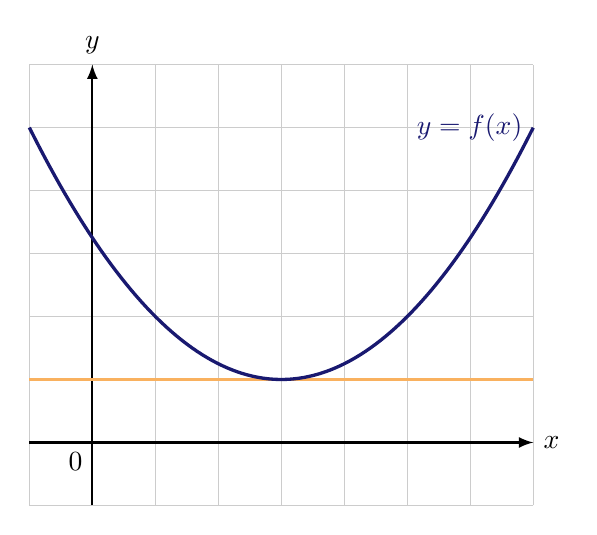
\begin{tikzpicture}[scale=0.8]
        \draw[thin,gray!40] (-1,-1) grid (7, 6);
        \draw[thick, ->, >=latex] (-1,0)--(7,0) node[right]{\(x\)};
        \draw[thick, ->, >=latex] (0,-1)--(0,6) node[above]{\(y\)};
        \draw (0, 0) node[below left] {0};

        \draw[BurntOrange!60, very thick] (-1, 1) -- (7, 1);

        \draw [MidnightBlue, very thick, domain=-1:7, samples=100] plot (\x,{0.25*(\x-3)^2+1}) node[left, MidnightBlue] {\(y = f(x)\)};
    \end{tikzpicture}
    
    \caption{At a local minimum, the derivative of a function is zero.}
    \label{fig:Ch06-local-minimum}
\end{figure}


\begin{figure}[H]
    \centering

    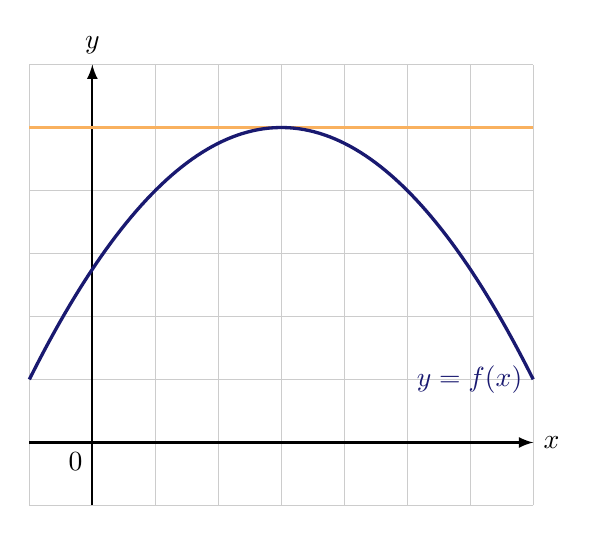
\begin{tikzpicture}[scale=0.8]
        \draw[thin,gray!40] (-1,-1) grid (7, 6);
        \draw[thick, ->, >=latex] (-1,0)--(7,0) node[right]{\(x\)};
        \draw[thick, ->, >=latex] (0,-1)--(0,6) node[above]{\(y\)};
        \draw (0, 0) node[below left] {0};

        \draw[BurntOrange!60, very thick] (-1, 5) -- (7, 5);

        \draw [MidnightBlue, very thick, domain=-1:7, samples=100] plot (\x,{-0.25*(\x-3)^2+5}) node[left, MidnightBlue] {\(y = f(x)\)};
    \end{tikzpicture}
    
    \caption{At a local maximum, the derivative of a function is zero.}
    \label{fig:Ch06-local-maximum}
\end{figure}


\begin{figure}[H]
    \centering

    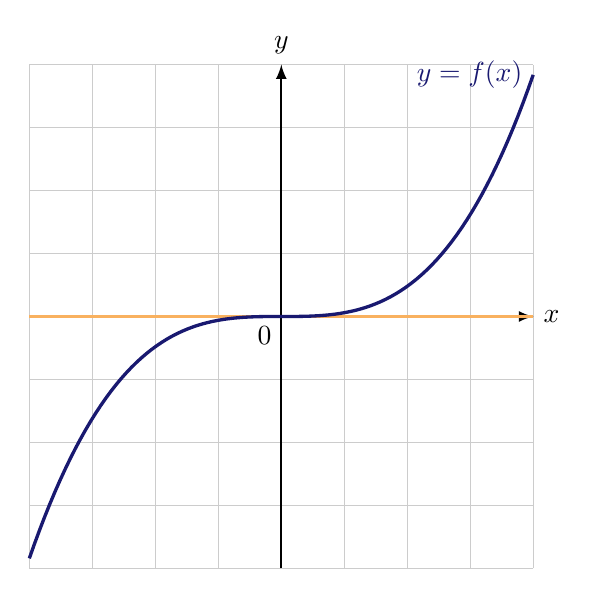
\begin{tikzpicture}[scale=0.8]
        \draw[thin,gray!40] (-4,-4) grid (4, 4);
        \draw[thick, ->, >=latex] (-4,0)--(4,0) node[right]{\(x\)};
        \draw[thick, ->, >=latex] (0,-4)--(0,4) node[above]{\(y\)};
        \draw (0, 0) node[below left] {0};

        \draw[BurntOrange!60, very thick] (-4, 0) -- (4, 0);

        \draw [MidnightBlue, very thick, domain=-4:4, samples=100] plot (\x,{0.06*(\x)^3}) node[left, MidnightBlue] {\(y = f(x)\)};
    \end{tikzpicture}
    
    \caption{At an inflection point, the derivative of a function is zero.}
    \label{fig:Ch06-inflection-point}
\end{figure}

There are several ways to distinguishing between these cases, as will be demonstrated using the following function.
%
\[f(x) = 2x^3 - 9x^2 + 12x - 4\]
%
To find the stationary points of \(f\), we first compute its derivative and set it equal to zero.
%
\begin{align*}
    f'(x) = 6x^2 - 18x + 12 &= 0\\
    x^2 - 3x + 2 &= 0\\
    (x - 1)(x - 2) &= 0\\
    x &= 1 \text{ or } 2
\end{align*}
%
This means that this function has two stationary points: one at \(x = 1\) and one at \(x = 2\). But are these local maxima, local minima, or inflection points?

One straightforward way for working this out is the \textit{first derivative test}, where we consider the sign of the derivative around the stationary point.

\begin{center}
    \begin{tabular}{|c||c|c|c|c|c|}
        \hline
        \(x\) & \(0\) & \(1\) & \(1.5\) & \(2\) & \(3\)\\
        \hline
        \(f'(x)\) & \(+\) & \(0\) & \(-\) & \(0\) & \(+\)\\
        \hline
    \end{tabular}
\end{center}

We can infer from the table above that \(f\) has a local maximum at \(x = 1\) and a local minimum at \(x = 2\), which can be verified using a graph.


\begin{figure}[H]
    \centering

    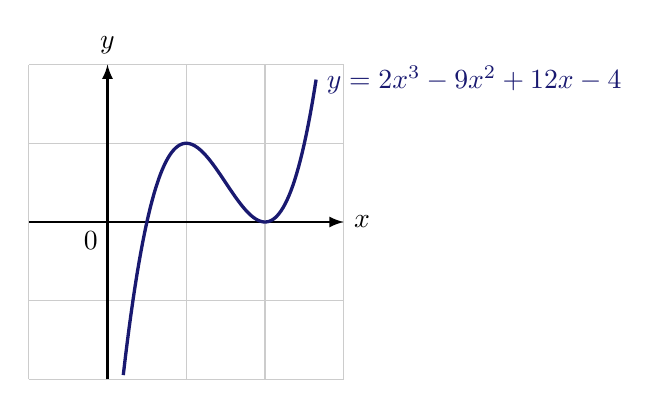
\begin{tikzpicture}[scale=1]
        \draw[thin,gray!40] (-1,-2) grid (3, 2);
        \draw[thick, ->, >=latex] (-1,0)--(3,0) node[right]{\(x\)};
        \draw[thick, ->, >=latex] (0,-2)--(0,2) node[above]{\(y\)};
        \draw (0, 0) node[below left] {0};

        \draw [MidnightBlue, very thick, domain=0.2:2.65, samples=100] plot (\x,{2*(\x)^3-9*(\x)^2+12*\x-4}) node[right, MidnightBlue] {\(y = 2x^3 - 9x^2 + 12x - 4\)};
    \end{tikzpicture}
    
    \caption{The function \(f(x) = 2x^3 - 9x^2 + 12x - 4\) has a local maximum at \(x = 1\) and a local minimum at \(x = 2\).}
    \label{fig:Ch06-stationary-point-example}
\end{figure}


Another way to identify the nature of a stationary point is the \textit{second derivative test}. This involves computing the second derivative of the function at each stationary point.
%
\begin{itemize}
    \item If the second derivative is positive, then the function has a local minimum at that point.
    \item If the second derivative is negative, then the function has a local maximum at that point.
    \item If the second derivative is zero, then the test is inconclusive. The point can be a local maximum, a local minimum, or an inflection point.
\end{itemize}
%
Applying this test to the function above, we have
%
\[f''(x) = 12x - 18\]
%
which gives us
%
\begin{align*}
    f''(1) &= -6 < 0\\
    f''(2) &= 6 > 0
\end{align*}
%
This leads to the same result as before: \(f\) has a local maximum at \(x = 1\) and a local minimum at \(x = 2\).



\subsection{Differential equations}

Differential equations are ones that involve both functions and their derivatives. Recall from earlier that a function of the form
%
\begin{equation*}
    f(x) = c \cdot e^{g(x)}
\end{equation*}
%
must have the derivative
%
\[f'(x) = c \cdot e^{g(x)} \cdot g'(x) = f(x) \cdot g'(x)\]
%
where \(c \in \mathbb{R}\). We will make use of this relationship a lot when solving differential equations, as we will see in the following example problems.

\vspace{15pt}
\begin{mdframed}[linewidth=1pt]

\noindent \textbf{Problem.} Solve \(f(x) = f'(x)\).

\textbf{Solution.} \(f(x) = C \cdot e^x\) where \(C \in \mathbb{R}\).

\vspace{2pt}
\end{mdframed}

\vspace{15pt}
\begin{mdframed}[linewidth=1pt]

\noindent \textbf{Problem.} Solve \(f'(x) = -3f(x)\).

\textbf{Solution.} \(f(x) = C \cdot e^{-3x}\) where \(C \in \mathbb{R}\).

\vspace{2pt}
\end{mdframed}

Now consider the slightly more complicated case of having to solve
%
\[f'(x) = a(x) \cdot f(x)\text{.}\]
%
To do this, we find the primitive (antiderivative) of \(a(x)\), which we will denote \(A(x)\). In other words, we have \(A'(x) = a(x)\). The solutions to this differential equation are then given by \(f(x) = C \cdot e^{A(x)}\), where \(C \in \mathbb{R}\). An example is given below.

\vspace{15pt}
\begin{mdframed}[linewidth=1pt]

\noindent \textbf{Problem.} Solve \(f'(x) = (2x+1) \cdot f(x)\).

\textbf{Solution.} The antiderivative of \(2x + 1\) is \(x^2 + x\), so the solution to the equation is given by \(f(x) = C \cdot e^{x^2 + x}\) where \(C \in \mathbb{R}\).

\vspace{2pt}
\end{mdframed}

These solutions, which contain unspecified multiplicative constants, are called \textit{general solutions} of the differential equation. Sometimes we might be asked to find specific values for these constants by using initial conditions.

\vspace{15pt}
\begin{mdframed}[linewidth=1pt]

\noindent \textbf{Problem.} What is the solution of \(f'(x) = (2x+1) \cdot f(x)\) that verifies \(f(0) = 3\)?

\textbf{Solution.} Continuing from the previous example problem, we know that the solution to the differential equation is given by \(f(x) = C \cdot e^{x^2 + x}\), where \(C \in \mathbb{R}\). We can find the value of \(C\) by using the initial condition \(f(0) = 3\).
%
\begin{align*}
    C \cdot e^{0^2 + 0} &= 3\\
    C &= 3
\end{align*}

This gives us the specific solution \(f(x) = 3 \cdot e^{x^2 + x}\).

\vspace{2pt}
\end{mdframed}

